In this chapter, we will talk about the implementation of our experiment. The details of the pipeline architecture, and the techniques used to obtain and curate data are unveiled. Details on the data munging and preprocessing are also given. The backend was implemented in Python, while the clients are implemented in javascript.\\

\section{Ingest}

We built a system to ingest the images from the NOAA service. It lazily downloads the images by checking first if the file is already present in the temporary folder. If the file does not exist it downloads it, then the system tries to add it to the database and persistent file system. To maintain a coherent one to one mapping between the database and the file system, the process of adding a new scene must be successful both in the database and in the filesystem, otherwise, the file is erased from both, and the state of the system remains as it was before the ingestion attempt.\\

\section{Tag}

Aerial tagged data is scarce. In particular, for the purpose of our experiment, we don't have any useful metadata on the images. We propose a method to tag samples of the scenes using crowd sourcing. We built a service that crops samples from the images and exposes them to an online application that lets any user with access to tag an image. We have three categories: the image has water in it, the image does not have water in it, and it is not possible to tell. When a positive answer is obtained, the system persists de image in the data base with the information of from which scene was it extracted.\\


\section{Data augmentation}

Given the nature of our task, it is hard to acquire the tagged images. To increment the size of our training dataset, even more, we use a technique known as data augmentation. It relies on the fact that affine transformations do not change the content of the scenes, however, a transformed scene appears as a completely new one to the classifier.\\

The images were rotated by 10 degrees, and reflected by the x-axis and the y-axis this gives us a $x144$ factor, this means that for each tagged image, the training corpus is incremented by $144$ images. The problem with this approach is that when a square image is rotated, some information on the corners is lost so we have to adjust the original image so that we can still crop a complete square from the desired size from it. For our experiment, the input size for the neural network is $227\times 227$ pixels, so the original images must be at least $\sqrt{2}$ times $227$ on each side. This way no matter how we rotate the original image, we can still crop a $227\times 227$ from the center of the rotation without losing any data.\\

\section{Database}

In the figure we show a subset of the database diagram. Tables inherent to the features of the django framework are not shown. The database design was based on reproducible reaseach. We wanted to keep track of the charactistics of the models trained. Also we wanted to know which where the training images used for each model. In order for the tagging application to work, images must be ingested into the system so every time a new sample is tagged we populate the database with information about the original image and the coordinates relative to the original image. In the final stage of the process we produce a list of potential damaged buildings which are also inserted into the database with geografical information and human readable address. We think that this can be helpfull to allocate resources in the most efficient way.

\begin{figure}[h]
  \begin{center}
    \subfigure{\label{fig:database}\fbox{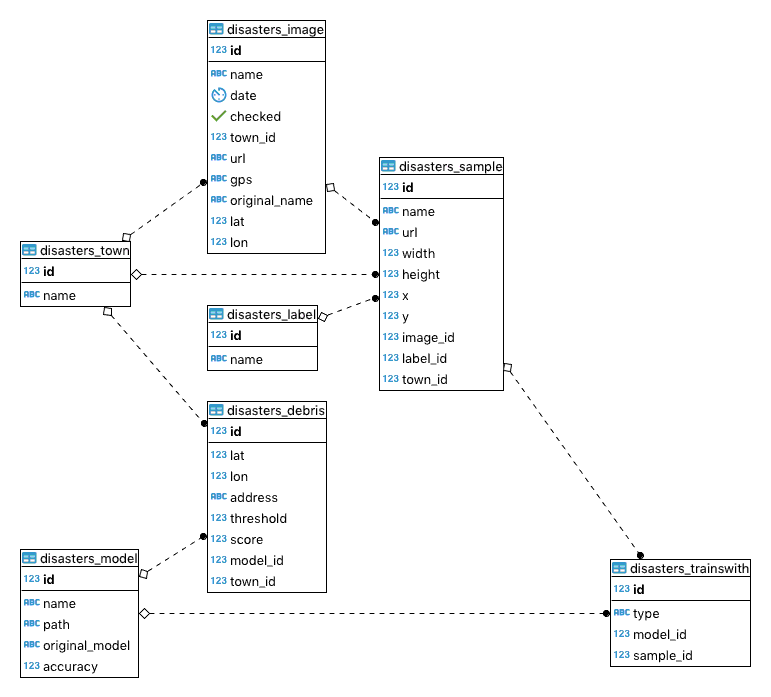
\includegraphics[width=1\textwidth]{images/database.png}}}
  \end{center}
\end{figure}

\section{Train}

We needed data to train our model. Raw dron images where obtained from the National Center for Disaster Prevention (CENAPRED). Drons flew over three towns in the state of Oaxaca producing $3733$ images during several days. Images contain gps information about the place where they where taken, however, it is not posible to produce a one to one mapping from the pictures to georeferenced points. With this limitation it was not possible to locate possible damaged buildings from the raw images. However, the model does not need any geografical information to be trained as it relies only in the pixel intensities.

Cropping and tagging manualy a large number of samples from the images was prohibitive. In order to overcome this obstacle an online tagging application was developed for this purpose. The idea was to decentralize the tagging procedure by giving an easy to use tool that was able to run from any browser. This way the cumbersome task of tagging the images can be crowdsourced.

By consuming the REST api described in the previous section, a simple web client was developed using jquery and openlayers. The interface is an image viewer with a selection and a button to submit an opition on that the higlighted area. The user will select an appropiate section of the given image, tag it, and then submit the section. In the backend, the image is cropped and ingested into the database.

\begin{figure}[h]
  \begin{center}
    \subfigure{\label{fig:database}\fbox{\includegraphics[width=1\textwidth]{images/visualise.png}}}
  \end{center}
\end{figure}

An additional button is given that lets the user see how well is the current best model performing. The process is quite similar to the previous one. In the server, the image is cropped and then the thumbnail is exposed to the model and the result is written back to the client through the REST api.

\begin{figure}[h]
  \begin{center}
    \subfigure{\label{fig:database}\fbox{\includegraphics[width=1\textwidth]{images/predict.png}}}
  \end{center}
\end{figure}


\begin{figure}[h]
  \begin{center}
    \subfigure{\label{fig:database}\fbox{\includegraphics[width=1\textwidth]{images/submit.png}}}
  \end{center}
\end{figure}

During the process, we noticed that the tagging process can lead to errors. In order to deal with those mistaken tagged images, a visualiser for the tagged images was developed. It consist in a simple interface where the last tagged images are shown with their respective tag. The interface offers a way to delete a given image or just edit the previously assigned tag.

\begin{figure}[h]
  \begin{center}
    \subfigure{\label{fig:database}\fbox{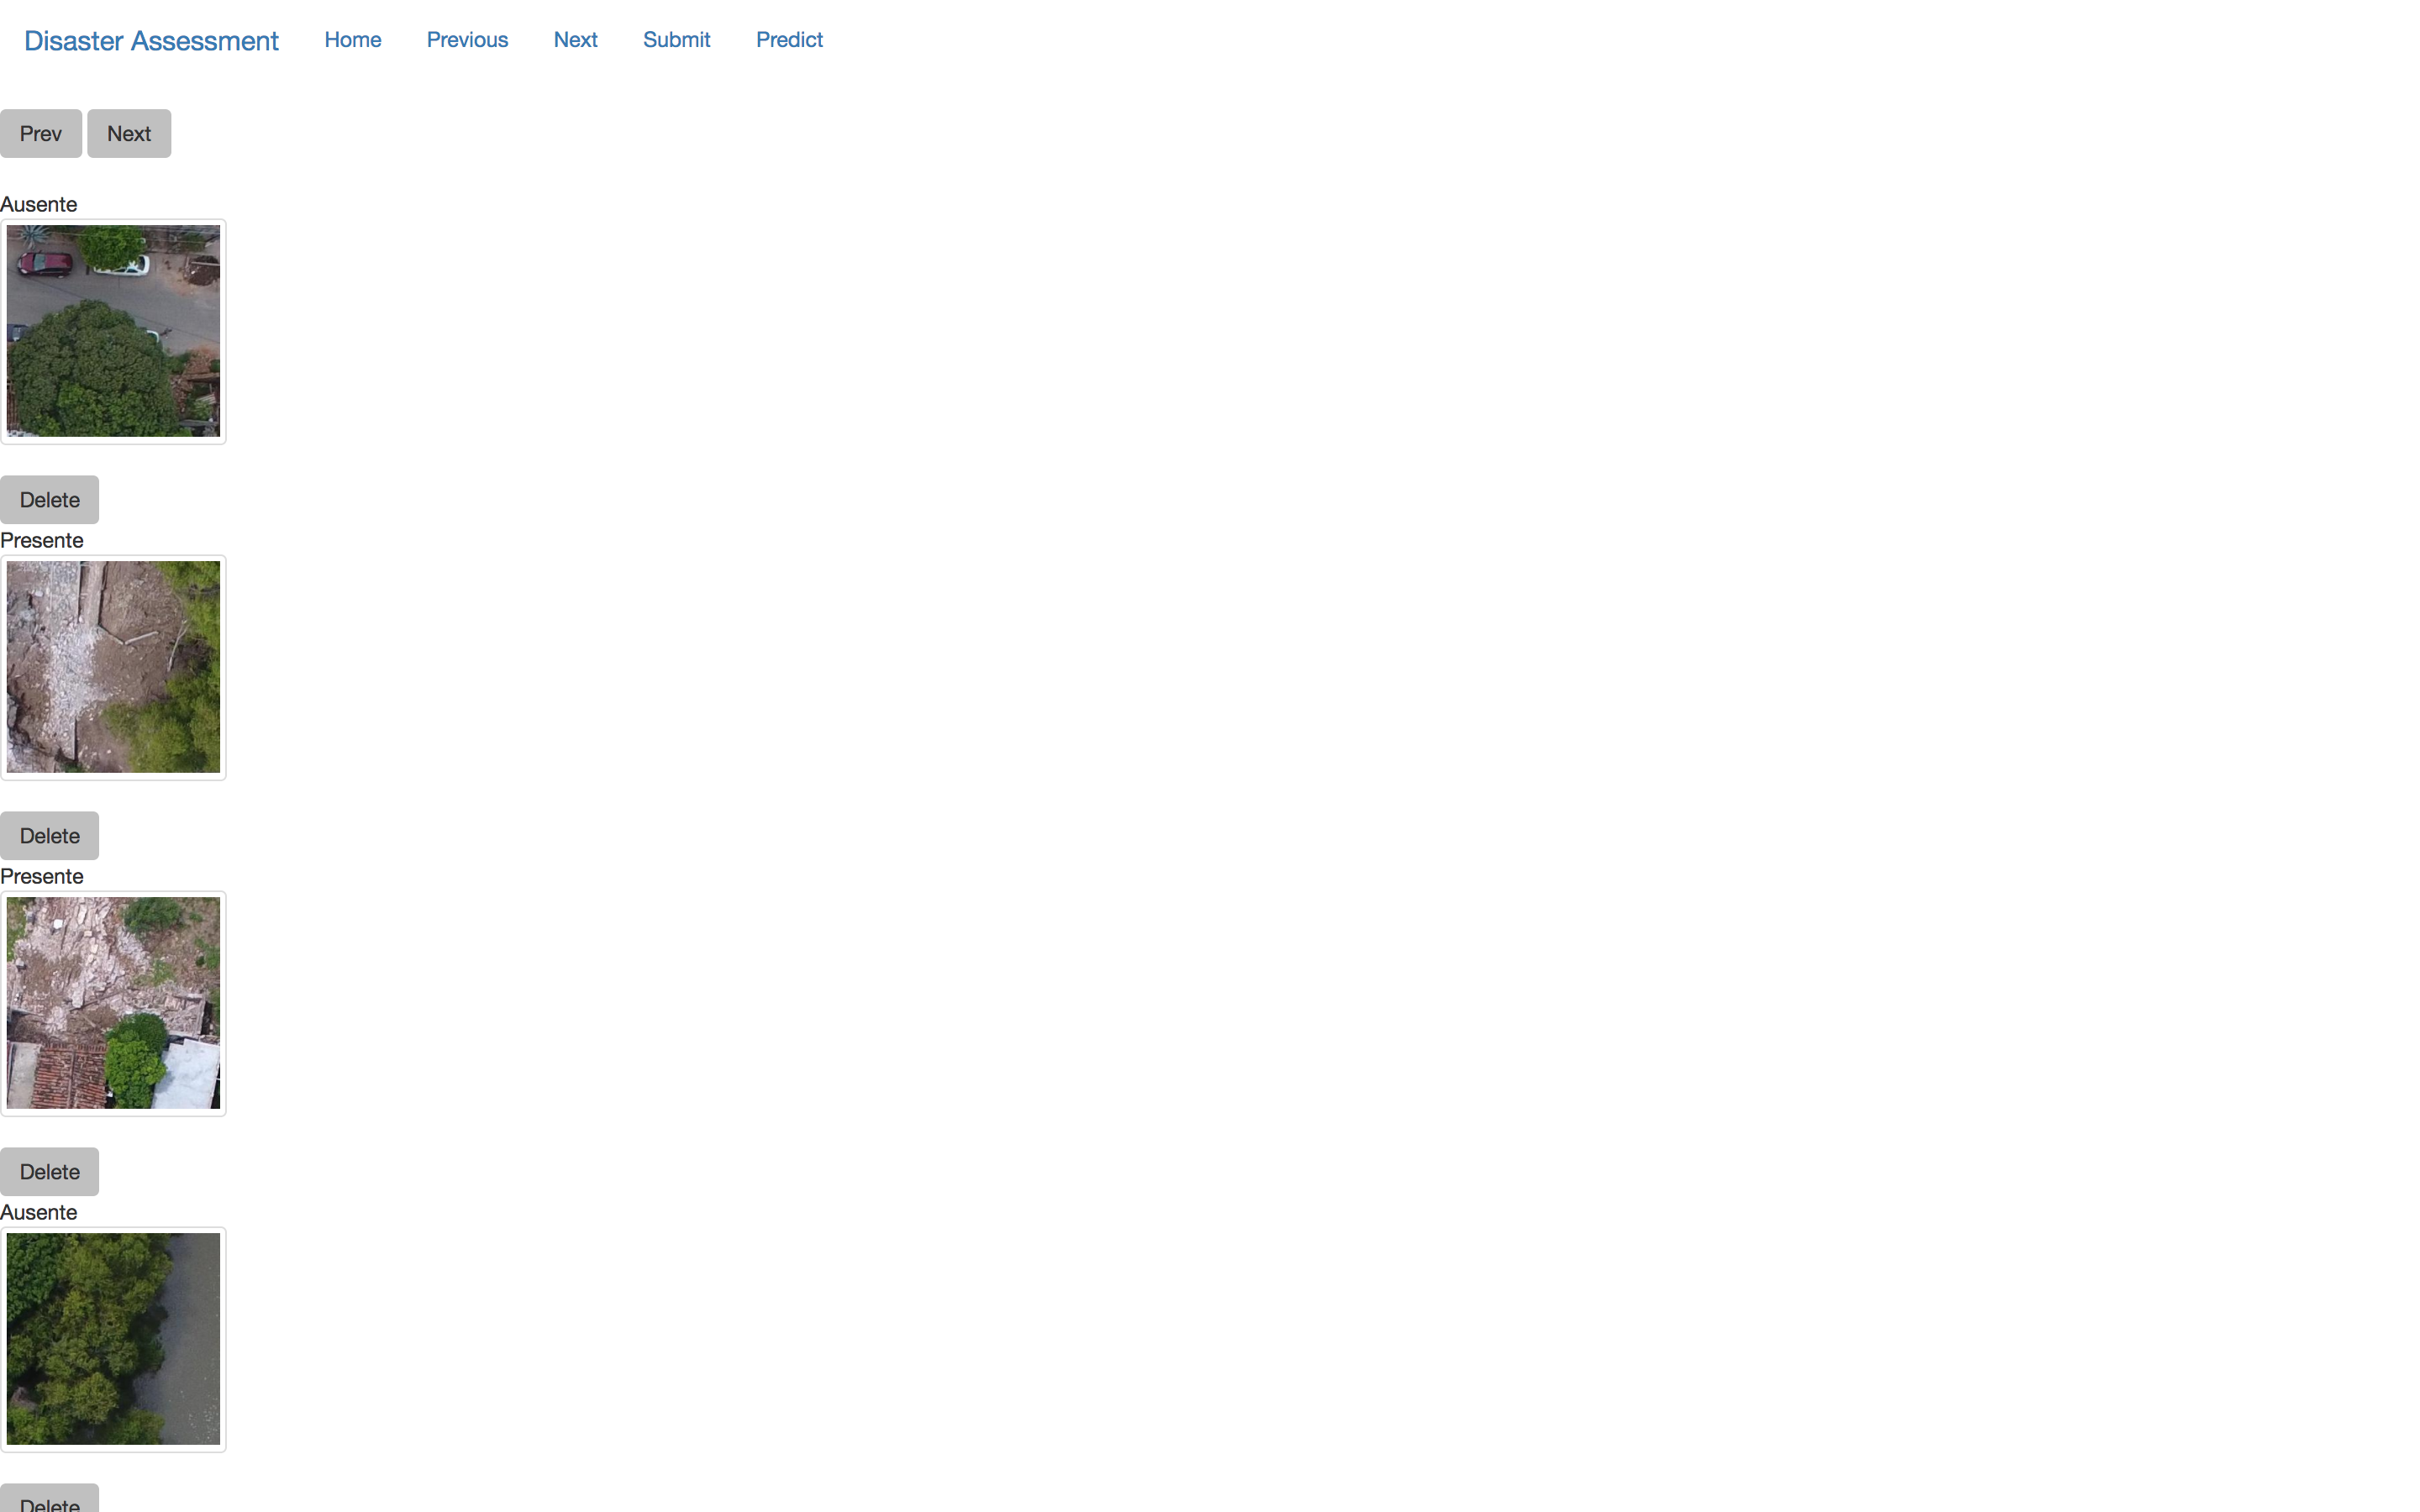
\includegraphics[width=1\textwidth]{images/thumbnails.png}}}
  \end{center}
\end{figure}
Finally, we developed a view for the points that the algorithm finds in the ortorectified image. This view was implemented with open layers and shows information about the location of the potential damaged building in a human readable form. This is done by querying the google api with the latitude and longitude points extracted from the map.

\begin{figure}[h]
  \begin{center}
    \subfigure{\label{fig:database}\fbox{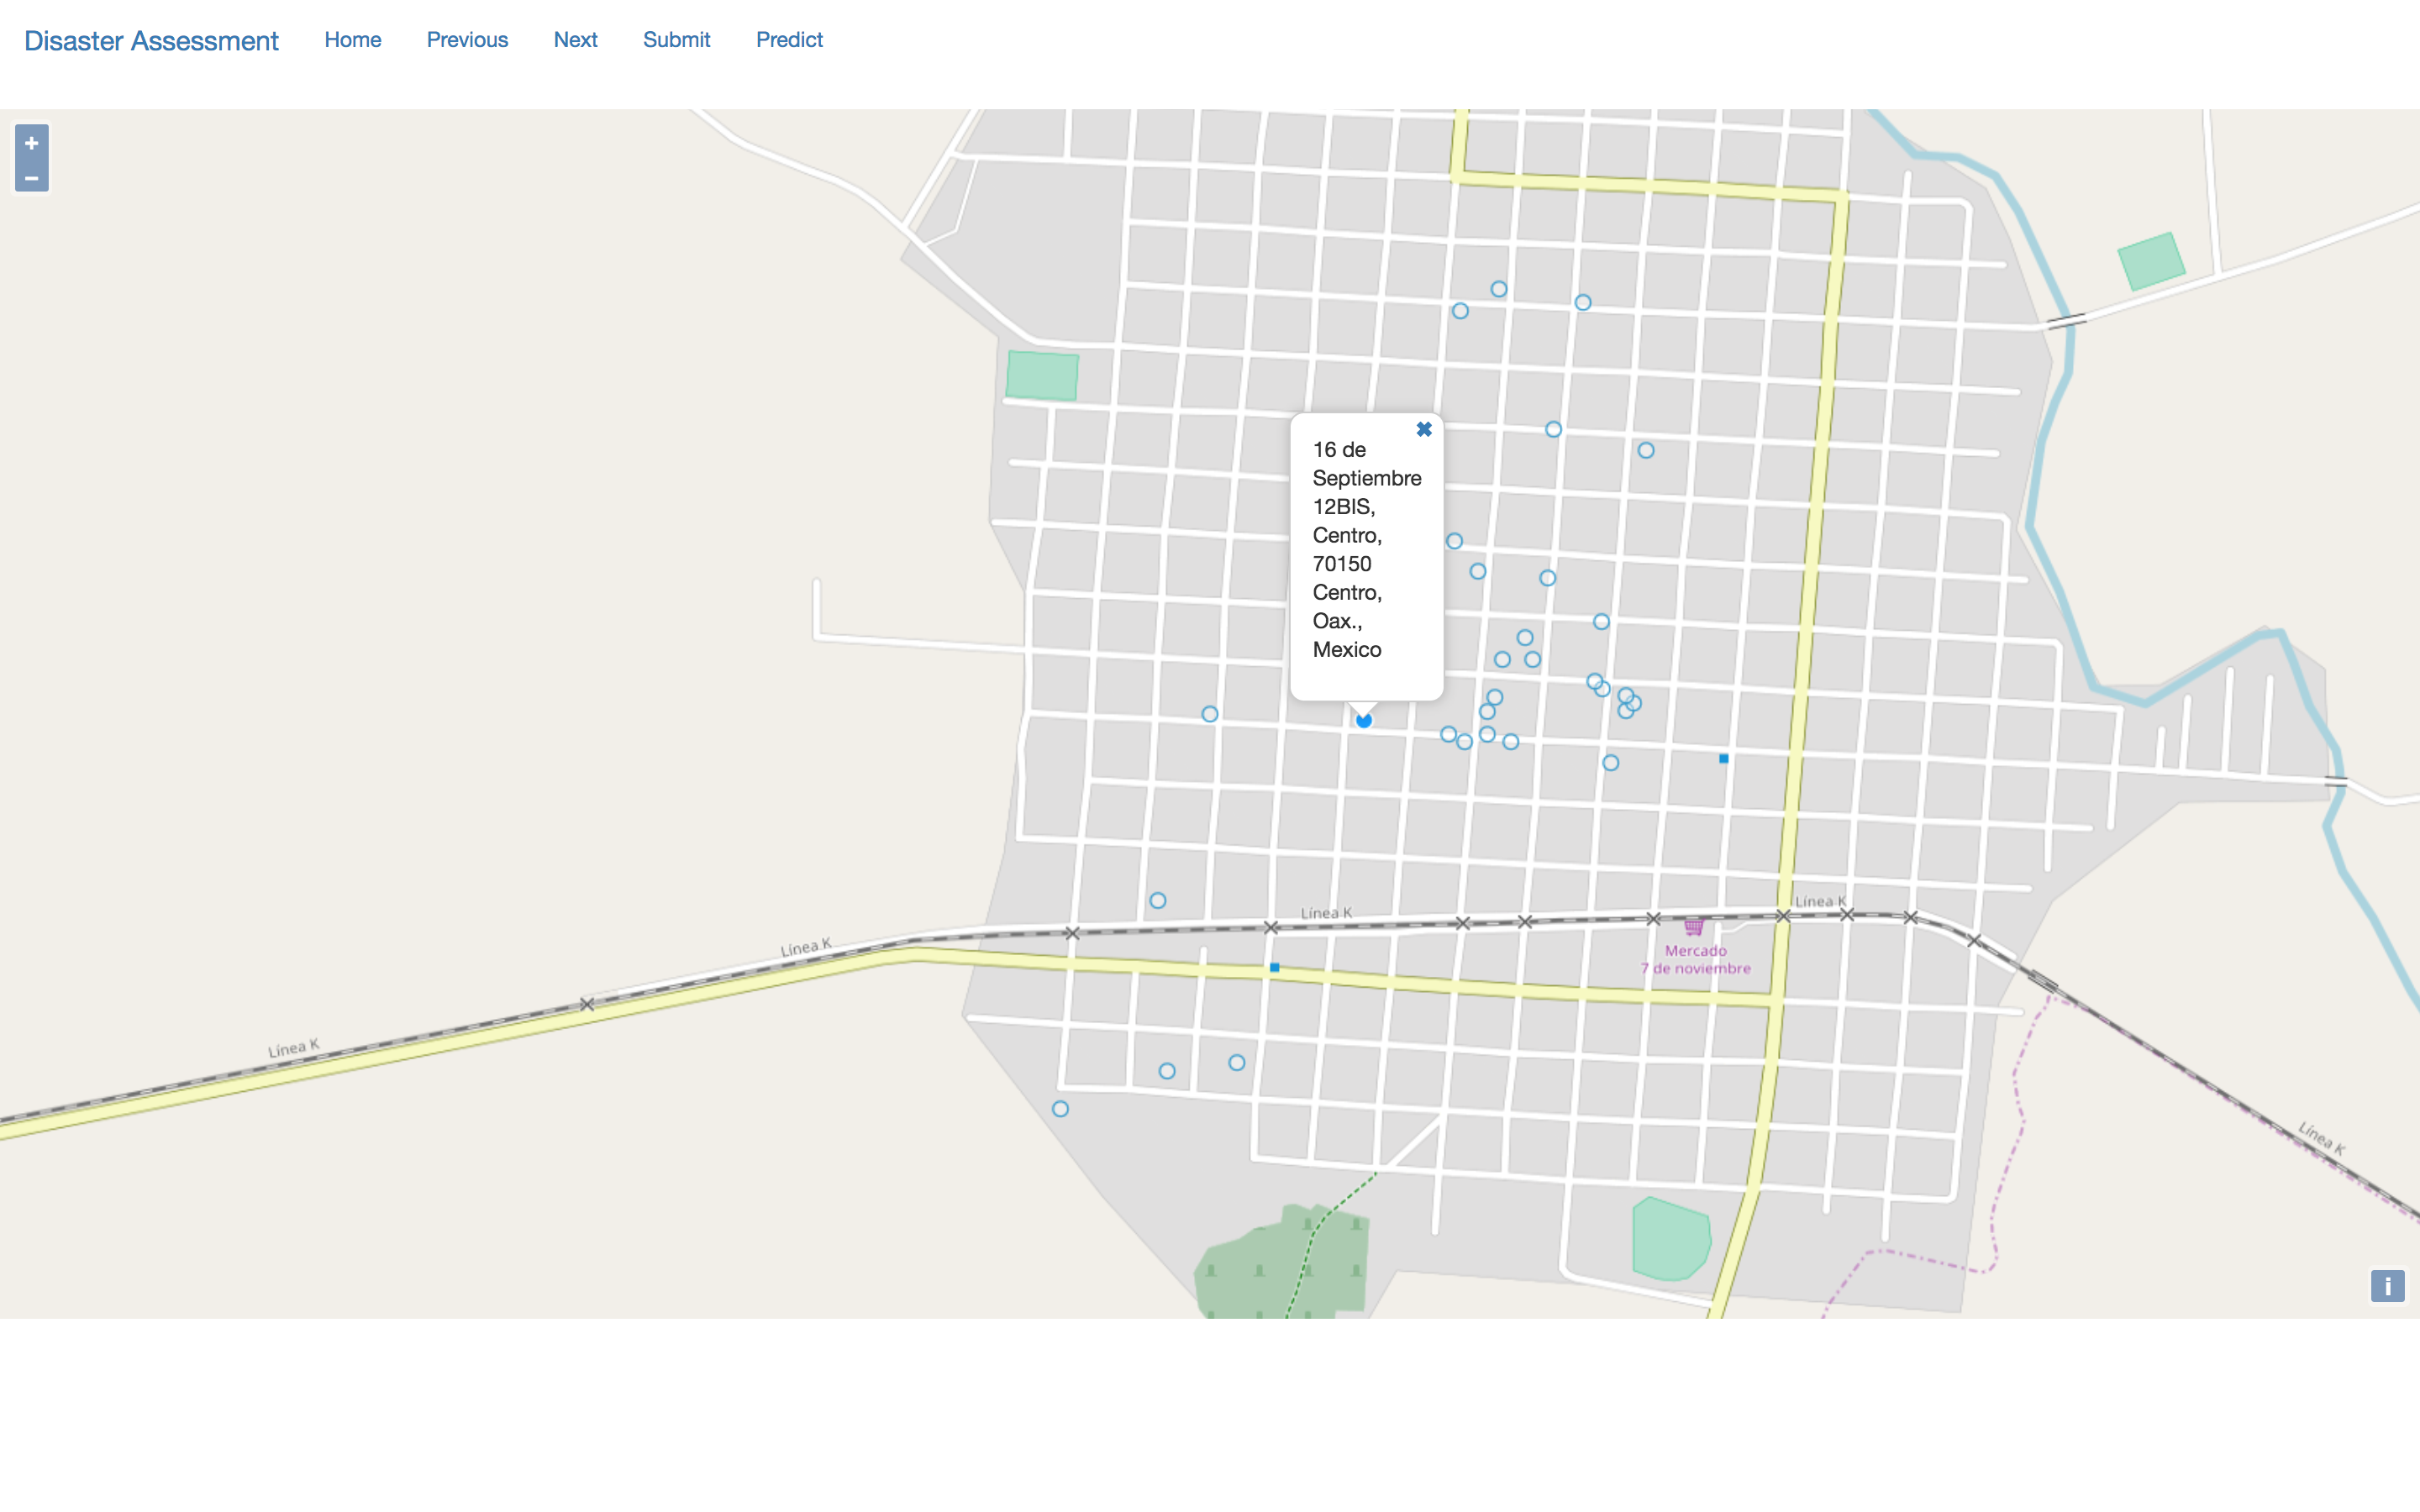
\includegraphics[width=1\textwidth]{images/debris.png}}}
  \end{center}
\end{figure}

\section{Predict}

Another simple front end application was developed to predict on new features, it is very similar to the tagging application. Instead of asking the user about the correct tag, it queries the model and exposes the answer to the front end.\\



\section{Model creation}

In order to create the model we need to select a sample from the thumbnails that we extracted from the original images. We wanted to create a process that was easily reproductible so we would compare models in a simple fashion. To this end the sample must be random each run and we need to split the images in three sets: training, validation and testing.\\

Tensorflow provides a script to retrain the last layer of inception by conecting the extracted features into a sofmax layer, and then training this classifier on the given set. It requires a directory layout tailored built to this purpose. The script was modified to fit our database design in order to make as easy as possible to train several models with homogeneous training, validation, and testing sets.


